% Fig.: simulated crashes per checkpoint in the stress runs (report/data/stress.json), in the
% order the checkpoints are reached.
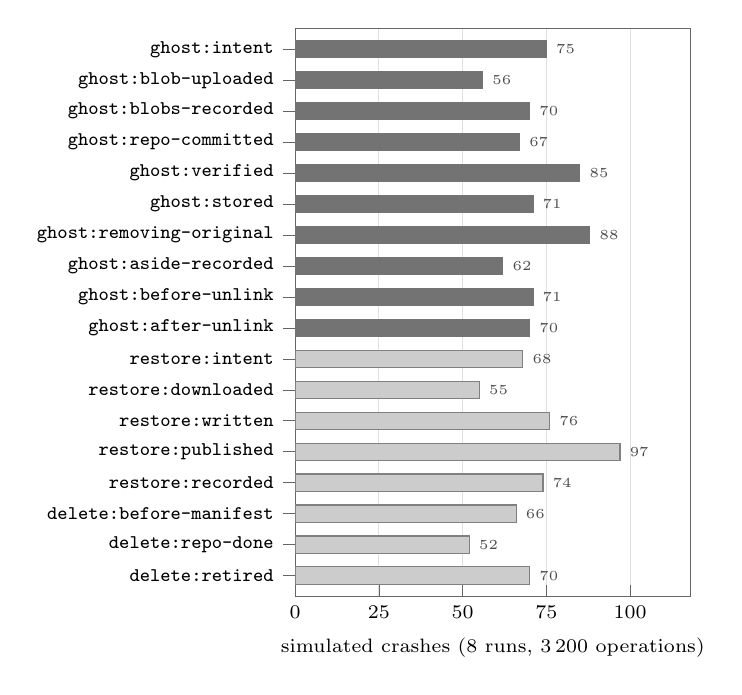
\begin{tikzpicture}
\begin{axis}[
  xbar, bar shift=0pt, width=66mm, height=88mm,
  font=\scriptsize,
  bar width=2.2mm,
  xmin=0, xmax=118, xtick={0,25,50,75,100},
  xlabel={simulated crashes (8 runs, 3\,200 operations)},
  y dir=reverse, enlarge y limits=0.04,
  ytick={ghost:intent, ghost:blob-uploaded, ghost:blobs-recorded, ghost:repo-committed,
                     ghost:verified, ghost:stored, ghost:removing-original, ghost:aside-recorded,
                     ghost:before-unlink, ghost:after-unlink, restore:intent, restore:downloaded,
                     restore:written, restore:published, restore:recorded, delete:before-manifest,
                     delete:repo-done, delete:retired},
  xtick pos=bottom, ytick pos=left,
  symbolic y coords={ghost:intent, ghost:blob-uploaded, ghost:blobs-recorded, ghost:repo-committed,
                     ghost:verified, ghost:stored, ghost:removing-original, ghost:aside-recorded,
                     ghost:before-unlink, ghost:after-unlink, restore:intent, restore:downloaded,
                     restore:written, restore:published, restore:recorded, delete:before-manifest,
                     delete:repo-done, delete:retired},
  yticklabel style={font=\scriptsize\ttfamily},
  axis line style={black!60}, tick style={black!60},
  xmajorgrids, grid style={black!12},
  nodes near coords, nodes near coords style={font=\tiny, text=black!70, anchor=west},
]
\addplot[fill=black!55, draw=black!55] coordinates {
  (75,ghost:intent) (56,ghost:blob-uploaded) (70,ghost:blobs-recorded) (67,ghost:repo-committed)
  (85,ghost:verified) (71,ghost:stored) (88,ghost:removing-original) (62,ghost:aside-recorded)
  (71,ghost:before-unlink) (70,ghost:after-unlink)};
\addplot[fill=black!20, draw=black!50] coordinates {
  (68,restore:intent) (55,restore:downloaded) (76,restore:written) (97,restore:published)
  (74,restore:recorded) (66,delete:before-manifest) (52,delete:repo-done) (70,delete:retired)};
\end{axis}
\end{tikzpicture}
